\chapter{Methodology}
\label{ch:methodology}

\section{Overview}
In this chapter I walk through how I designed the Logic Advocate Tutor before writing a single line of production code. I cover the abstractions I built to bridge formal argumentation theory and an actual chat style interface, and the reasoning I used to pick one approach over another. In the next chapter I show the Python that brought all of this to life.

I can sum up my core problem in one sentence. I needed a debate environment where any natural language argument is forced to follow the same survival rules that a formal argumentation framework would apply, while still feeling responsive enough to behave like a normal chat app. To pull this off, I had to make the system do four jobs at once. It accepts free text arguments from a human or a Large Language Model. It maps those arguments into a directed graph of attacks and supports. It computes a real time acceptability score for every node. And it shows the result of that score back to the participants in a way that actually changes how they play their next move.

That is why I broke the system into four cooperating layers. I built a \textbf{Presentation Layer} for the UI and the visual feedback, a \textbf{Dialogue Layer} that enforces the rules of the game, a \textbf{Logic Layer} that holds the framework and runs the gradual semantics, and an \textbf{AI Layer} that talks to the LLM and turns its replies back into valid argument moves. Figure~\ref{fig:layered_arch} shows how the layers depend on each other. Each layer only knows about the layer below it. I made that isolation deliberate so I could swap out the language model, or rip out the UI, without breaking the math.

\section{Design Goals and Non Goals}
\label{sec:goals}
Before I get to the architecture, I want to be upfront about which problems my system actually tries to solve, and which I left for someone else to deal with later. My goals all came out of the gaps I identified back in Chapter~\ref{ch:background}.

\textbf{Goal 1: Keep the LLM honest.}
I noticed that a standalone LLM debate agent suffers from rhetorical rigidity \cite{ku2025multiagent} and tends to claim victory no matter what is actually happening in the debate \cite{aoyagui2025subjective}. So I needed my system to maintain its own ground truth view of the debate, computed by an algorithm I trust rather than by a model that sometimes lies for the sake of looking confident. I let the LLM produce text and score how persuasive an argument is, but I do not let it decide who is winning.

\textbf{Goal 2: Continuous scores, not pass or fail labels.}
Classical Dung style semantics declare every argument either \texttt{IN} or \texttt{OUT} \cite{dung1995acceptability}. I find that binary verdict fine for theory but useless for a learner. If a student's claim is just told it has been ``defeated'', they have no idea how close it was, what to fix, or whether one more support would have saved it. Following the gradual semantics literature \cite{cayrol2005graduality, amgoud2017gradual}, I gave every argument a continuous score between 0 and 1 so the learner can watch their argument get weaker rather than just being told it died.

\textbf{Goal 3: Make support a first class citizen.}
I see real classroom debate as collaborative, not just adversarial. People build on each other's points all the time. So I extended the basic attack relation with a parallel \emph{support} relation, the way bipolar argumentation handles it \cite{cayrol2005bipolar}.

\textbf{Goal 4: Different audiences value different kinds of arguments.}
In my view, a factual claim should hit harder against an emotional one than the other way around, at least if the audience is fact leaning. Following Bench-Capon's value based framework \cite{benchcapon2003value}, I added a value tag to every argument, and the tag scales the strength of attacks and supports across tags.

\textbf{Goal 5: Run anywhere, cost nothing.}
I needed my system to live inside a normal browser, take both text and voice, and let a student fire it up without any installation step. I also needed it to fit inside the free tier of every cloud service it touches, so a student can use it without a credit card.

\textbf{What I am not trying to do.}
My system does not do automatic argument mining from long essays \cite{wachsmuth2016essays}. It does not detect informal fallacies in your text. And it does not do the deep parsing I would need to extract Toulmin style warrants \cite{toulmin2003uses}. I treat each argument as a black box node, the way Dung treats them \cite{dung1995acceptability}. The framework does not look inside. The interesting bit is how I score those nodes, display them, and combine them with an LLM, not how their text gets parsed.

\section{The Four Layer Architecture}
\label{sec:architecture}
Figure~\ref{fig:layered_arch} shows the layers I built and what flows between them. A user move (text, voice, or an image) enters at the top and gets pushed downward. Recomputed scores and the AI's reply travel back up to the screen. The figure colours \textsc{Symbolic} components in gold (the Logic Layer and the Hint MDP) and \textsc{Neural} components in red (the AI Layer), so the boundary between deterministic Python and stochastic LLM is visible at a glance.

\begin{figure}[h]
\centering
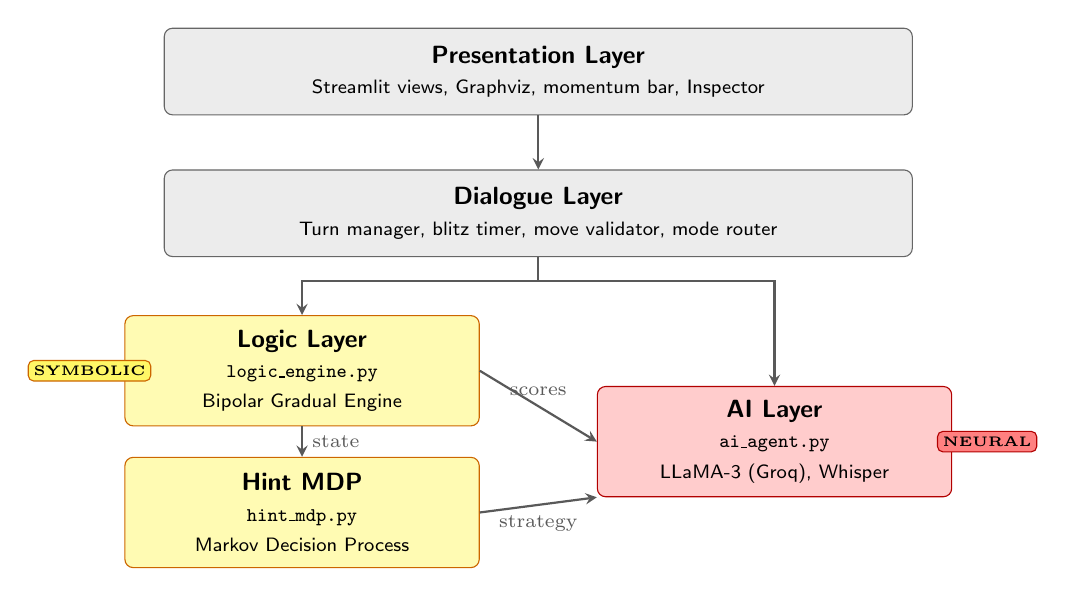
\begin{tikzpicture}[
    every node/.style={font=\small\sffamily, align=center},
    hybrid/.style={rectangle, draw=black!60, rounded corners=3pt,
                    fill=gray!15, minimum width=9.5cm, minimum height=1.1cm},
    symbolic/.style={rectangle, draw=orange!80!black, rounded corners=3pt,
                      fill=yellow!30, minimum width=4.5cm, minimum height=1.4cm},
    neural/.style={rectangle, draw=red!70!black, rounded corners=3pt,
                    fill=red!20, minimum width=4.5cm, minimum height=1.4cm},
    arr/.style={->, >=stealth, thick, gray!70!black},
]
\node[hybrid]   (pres) at (0, 0) {\textbf{Presentation Layer} \\ {\scriptsize Streamlit views, Graphviz, momentum bar, Inspector}};
\node[hybrid]   (dial) at (0, -1.8) {\textbf{Dialogue Layer} \\ {\scriptsize Turn manager, blitz timer, move validator, mode router}};
\node[symbolic] (logic) at (-3.0, -3.8) {\textbf{Logic Layer} \\ {\scriptsize \texttt{logic\_engine.py}} \\ {\scriptsize Bipolar Gradual Engine}};
\node[symbolic] (mdp)   at (-3.0, -5.6) {\textbf{Hint MDP} \\ {\scriptsize \texttt{hint\_mdp.py}} \\ {\scriptsize Markov Decision Process}};
\node[neural]   (ai)    at (3.0, -4.7) {\textbf{AI Layer} \\ {\scriptsize \texttt{ai\_agent.py}} \\ {\scriptsize LLaMA-3 (Groq), Whisper}};
\draw[arr] (pres) -- (dial);
\draw[arr] (dial.south) -- ++(0, -0.3) -| (logic.north);
\draw[arr] (dial.south) -- ++(0, -0.3) -| (ai.north);
\draw[arr] (logic.east) -- node[above, font=\scriptsize]{scores} (ai.west);
\draw[arr] (logic.south) -- node[right, font=\scriptsize]{state} (mdp.north);
\draw[arr] (mdp.east) -- node[below, font=\scriptsize]{strategy} (ai.south west);
\node[font=\tiny\bfseries, draw=orange!80!black, fill=yellow!60, rounded corners=2pt, inner sep=2pt] at (-5.7, -3.8) {SYMBOLIC};
\node[font=\tiny\bfseries, draw=red!70!black, fill=red!50, rounded corners=2pt, inner sep=2pt] at (5.7, -4.7) {NEURAL};
\end{tikzpicture}
\caption{The four layer architecture. Symbolic components (gold) are deterministic Python: the engine and the hint MDP. Neural components (red) are the LLM-backed AI Layer. Hybrid (grey) layers handle conversation and presentation. The pedagogical guarantee is that the LLM never receives the engine's verdict, so it cannot lie about who is winning.}
\label{fig:layered_arch}
\end{figure}

\paragraph{Presentation Layer.}
This is the part the user actually sees. I made it capture whatever move the user is making, draw the chat history as colour coded bubbles, render the live argumentation graph through Graphviz \cite{ellson2002graphviz}, and show the running acceptability percentages. Because Streamlit \cite{streamlit2024} re runs the whole script every time the user clicks anything, I wrote this layer to be rebuildable from session state alone. There is no hidden DOM trickery in my code.

\paragraph{Dialogue Layer.}
This layer enforces the rules of the dialogue game I lay out in Section~\ref{sec:dialogue_game}. It owns the turn order, the optional 60 second blitz timer, the move validator, and the mode router that dispatches to one of three game modes (see Section~\ref{sec:modes}). All of this state lives inside Streamlit's session dictionary, so the layer is reactive but stateless across server restarts.

\paragraph{Logic Layer.}
This is where my formal argumentation actually runs. I exposed one class, \texttt{AcademicLogicEngine}, that takes arguments, attacks and supports, and produces a vector of acceptability scores. I designed the class to know nothing about the user, the LLM, or the network. I could pull it out of the project and unit test it on its own, which is exactly what I do in Section~\ref{sec:eval_logical} of the next chapter. The math behind it is in Section~\ref{sec:bipolar_engine}.

\paragraph{AI Layer.}
This one only kicks in when the user picks Human vs AI mode or AI vs AI mode. I set up its job as follows. It reads the chat transcript, writes a counter argument, scores both the human's argument and its own on a 1 to 25 scale, and picks a value tag for whatever it just produced. The output gets passed back up to the Dialogue Layer like an ordinary move and inserted into the graph by my Logic Layer.

\section{The Bipolar Gradual Engine}
\label{sec:bipolar_engine}
The mathematical heart of everything I built is a custom evaluator I wrote by mashing together four ideas from the argumentation literature. Bipolarity I took from Cayrol and Lagasquie-Schiex \cite{cayrol2005bipolar}. Gradual semantics I took from \cite{cayrol2005graduality, amgoud2017gradual}. Value based weighting I took from Bench-Capon \cite{benchcapon2003value}. And preference based normalisation I took from Amgoud and Cayrol \cite{amgoud2002reasoning}. In this section I give the formal version of the math. In the next chapter I show the Python that runs it.

\subsection{Framework definition}
I represent a debate as a tuple
\[
\mathcal{F} = \langle \mathcal{A}, \mathcal{R}_{\text{att}}, \mathcal{R}_{\text{sup}}, w, v \rangle,
\]
where $\mathcal{A}$ is a finite set of arguments, $\mathcal{R}_{\text{att}} \subseteq \mathcal{A} \times \mathcal{A}$ is an attack relation, $\mathcal{R}_{\text{sup}} \subseteq \mathcal{A} \times \mathcal{A}$ is a support relation, $w : \mathcal{A} \rightarrow \{1, 2, \dots, 25\}$ assigns each argument an integer weight, and $v : \mathcal{A} \rightarrow \mathcal{V}$ tags each argument with one of four value labels:
\[
\mathcal{V} = \{\textsc{Fact}, \textsc{Logic}, \textsc{Ethics}, \textsc{Emotion}\}.
\]
I associate each value tag with a multiplier I picked by hand, inspired by Bench-Capon's audience model \cite{benchcapon2003value}:
\[
\mu(\textsc{Fact})=1.2, \quad \mu(\textsc{Logic})=1.1, \quad \mu(\textsc{Ethics})=1.0, \quad \mu(\textsc{Emotion})=0.8.
\]

\subsection{The acceptability score}
\label{sec:score}
For every argument $a \in \mathcal{A}$ my engine computes an acceptability score $s(a) \in [0, 1]$. I define the score as the fixed point of the following update rule, computed by ten rounds of synchronous relaxation starting from $s^{(0)}(a) = 1$ for every argument:
\[
\alpha(a) = \sum_{(b,a) \in \mathcal{R}_{\text{att}}} s(b) \cdot w(b) \cdot \frac{\mu(v(b))}{\mu(v(a))},
\]
\[
\sigma(a) = \sum_{(b,a) \in \mathcal{R}_{\text{sup}}} s(b) \cdot w(b) \cdot \frac{\mu(v(b))}{\mu(v(a))},
\]
\[
s^{(t+1)}(a) = \min\!\left(\, 1, \frac{1 + \kappa \cdot \sigma(a)/\max(1, w(a))}{1 + \alpha(a)/\max(1, w(a))} \,\right),
\]
where $\kappa \in (0, 1]$ is a support coefficient I tuned by hand. I deployed the engine with $\kappa = 1/2$. The motivation for that choice and what it does to the score is the subject of Section~\ref{sec:support_coefficient}.

After the loop converges, I recover a coarse status label so the rest of the UI has something it can switch on:
\[
\text{status}(a) = \begin{cases} \texttt{IN} & \text{if } s(a) \geq 0.5, \\ \texttt{OUT} & \text{otherwise.} \end{cases}
\]

\subsection{Why I chose this formula}
The shape $\frac{1+\sigma}{1+\alpha}$ borrows the spirit of the h categorizer \cite{besnard2001logic}, which divides initial strength by attack strength. I generalised it to the bipolar case by adding a matching numerator for support. Three things made it the right pick for a tutoring system. First, I made the score bounded. The numerator and denominator both grow linearly, so $s(a)$ never escapes $[0, 1]$ once I cap it at 1. That keeps the colour gradient in my UI well defined. Second, I made the score sensitive to weight. Both the attacker's strength and the target's resilience scale by $w$, so a stronger argument really is harder to take down. That gives me the preference based behaviour from \cite{amgoud2002reasoning} without falling back on the brittle binary defeat rule of the prototype I describe in Section~\ref{sec:prototype}. Third, I made the score react to value tags. The ratio $\mu(v(b))/\mu(v(a))$ is exactly what Bench-Capon's audience model \cite{benchcapon2003value} predicts. An emotional appeal landing on a factual claim should be weaker than the other way around, and I find that exactly that behaviour falls out of my math.

\subsection{The support coefficient $\kappa$}
\label{sec:support_coefficient}
The textbook bipolar gradual rule treats attack and support symmetrically. In its purest form a supporter of weight $w$ exactly cancels an attacker of the same weight, and the score saturates at $1$ as soon as $\sigma(a) \geq \alpha(a)$. I tried that in an early deployment and found the saturation pedagogically harmful. In any balanced debate (every claim defended by a roughly equal supporter from the same side) the per-node acceptability dropped out of the picture: every surviving node read $100\%$, regardless of how many attacks it was actually absorbing. The map turned into a wall of identical green boxes, and the only signal the learner had left was the momentum bar.

The fix I settled on is a single multiplicative constant $\kappa$ in front of $\sigma$ in the numerator. With $\kappa = 1/2$, a supporter of equal weight only partially compensates its target's attacker. The behaviour I get is the following:
\begin{itemize}
    \item No attack ($\alpha = 0$): $s = 1 + \kappa\sigma/w$, capped at $1$. An unattacked argument still scores $1$.
    \item Balanced ($\sigma = \alpha$): $s = (1 + \kappa) / 2 = 0.75$. The claim survives the threshold but is visibly damaged.
    \item Dominant support ($\sigma \geq \alpha / \kappa = 2\alpha$): the score returns to $1$. Only a clearly heavier supporter restores full acceptance.
    \item No support ($\sigma = 0$): $s = 1/(1+\alpha/w)$, independent of $\kappa$. The classical limit is therefore preserved exactly.
\end{itemize}

I am explicit that this is a departure from the published bipolar formula. I chose to keep it because the every-node-100\% mode was making the live demo of the system actively misleading, and the cost of the deviation, a $25$ percentage point reduction at the balanced case, gives the learner usable visual feedback. The single constant also localises the deviation: setting $\kappa$ back to $1$ recovers the textbook formula without any other code change. The trade-off shows up in my evaluation in Chapter~\ref{ch:results} as a softer support ablation: disabling supports now flips fewer verdicts than under $\kappa = 1$, because every support was contributing less to begin with.

\subsection{Relationship to classical Dung}
\label{sec:relationship_dung}
If I turn off the support relation ($\mathcal{R}_{\text{sup}} = \varnothing$), set every weight to 1, and only use one value tag, my gradual rule collapses exactly to the h categorizer of \cite{besnard2001logic}. Note that the support coefficient $\kappa$ from Section~\ref{sec:support_coefficient} multiplies $\sigma$, so with $\sigma = 0$ it drops out and the classical limit is independent of $\kappa$. In that special case an isolated argument has score 1, an argument hit by a single fully accepted attacker drops to 0.5, and the cascade approximates the grounded extension of \cite{dung1995acceptability} once I threshold at 0.5. So on classical inputs my engine behaves like a classical evaluator, and only departs from it when bipolar, weighted, or valued inputs make the binary world too coarse to be useful.

\subsection{From the prototype to the deployed engine}
\label{sec:prototype}
My repository still holds an early sketch of the engine in \texttt{class~Argument.txt}. That version used a strict preference based rule. An attacker only counted if its weight was at least the target's, otherwise the attack was silently dropped. This is the rule from Amgoud and Cayrol \cite{amgoud2002reasoning}. It looked clean on paper but I found it too brittle in practice. The LLM would sometimes fire off a weak but rhetorically clever attack against a heavyweight claim, and my prototype would just refuse to register the move. The user saw nothing happen. From a learning standpoint I judged that awful, because the disagreement disappears instead of being made visible. So in my deployed engine I softened the rule into the continuous ratio above. A weaker attacker still chips away at the target a little, but cannot drive its score below $1/(1+\alpha)$. The learner sees the attack land and can decide how worried to be.

\section{Hint Generation as a Markov Decision Process}
\label{sec:mdp}
The hint button does not just ask the LLM ``what should I do next?''. I wrap it in a formal Markov Decision Process so the LLM only writes the prose for a hint strategy that a policy chose under a verifiable reward function. The reward is tied to the engine's verdict on the learner's main claim, which is the same gradual semantics from Section~\ref{sec:score}. So when the learner gets a hint, the strategy behind it is a function of the formal state of the debate, not of what the LLM happens to think.

I model the hint system as the standard MDP tuple
\[
\langle S, A, P, R, \gamma \rangle.
\]

\paragraph{State space $S$.} I encode the learner's situation as a triple
\[
\text{state} = \big(\text{own\_status},\; \text{opponent\_pressure},\; \text{hint\_streak}\big),
\]
with $\text{own\_status} \in \{\textsc{Winning}, \textsc{Tied}, \textsc{Losing}\}$ derived from the engine's IN/OUT verdict on the learner's main claim, $\text{opponent\_pressure} \in \{\textsc{Low}, \textsc{High}\}$ flagged \textsc{High} when the opponent's most recent argument has score $\geq 0.65$, and $\text{hint\_streak} \in \{0, 1, \geq\!2\}$ counting hints used since the learner's last actual move. This gives $|S| = 3 \cdot 2 \cdot 3 = 18$ discrete states.

\paragraph{Action space $A$.} Four hint strategies:
\begin{itemize}
    \item \textsc{Strategic\_Attack} attack the opponent's weakest premise
    \item \textsc{Defensive\_Reinforce} reinforce the learner's own main claim
    \item \textsc{Value\_Reframe} suggest changing the value tag to neutralise an attack
    \item \textsc{Step\_Back} suggest abandoning or restating the main claim
\end{itemize}

\paragraph{Transition probability $P$.} I encode an expert-informed initial transition model in a function that maps state-action pairs to probability distributions over next states. The model is parameterised by four intuitions: \textsc{Strategic\_Attack} helps most when the learner is \textsc{Losing}; \textsc{Defensive\_Reinforce} helps most when \textsc{Tied}; \textsc{Value\_Reframe} counters \textsc{High} opponent pressure; \textsc{Step\_Back} is the rescue action. A fatigue multiplier (matching the non-evaluative principle of Stamper et al.~\cite{stamper2011hints}) shrinks the landing probability of any second or third consecutive hint. The empirical re-estimation of $P$ from logged student trajectories is left as a stub in the codebase and listed as future work in Chapter~\ref{ch:conclusion}.

\paragraph{Reward function $R$.} This is the part that links the MDP back to the engine. After the learner's next actual move, the reward is
\[
R(s, a, s') = \begin{cases}
   +1 & \text{if } \text{own\_status}(s') = \textsc{Winning} \\
   \phantom{+}0 & \text{if } \text{own\_status}(s') = \textsc{Tied} \\
   -1 & \text{if } \text{own\_status}(s') = \textsc{Losing}
\end{cases}
\;-\; 0.05,
\]
where the constant $-0.05$ is the per-hint cost that follows Stamper's design recommendation of mildly discouraging hint-spamming without punishing legitimate help-seeking. \textbf{The reward is tied directly to the engine's logical-validity verdict.} It is not a function of any LLM output. This is the explicit answer to the requirement that the reward function be linked to the logical validity of the student's argument.

\paragraph{Discount $\gamma$.} I use $\gamma = 0.9$, the standard textbook value.

\paragraph{Solver.} The state space is small enough that I solve the MDP exactly by value iteration at module import time. The optimal policy $\pi^*: S \rightarrow A$ is cached, so a hint button click is constant time.

\section{The Implicit Premise Detector}
\label{sec:premise}
A small but novel feature on top of the engine is the implicit-premise detector. The diagnosis in Ku et al.~\cite{ku2025multiagent} is that LLMs (and humans) often skip the unstated assumption their reasoning rests on. I flipped that diagnosis into a UI feature. Before the learner submits an argument, they can click ``Check assumptions.'' The system sends the draft argument plus the last few moves of context to an LLM with an analytic prompt at temperature $0.4$ that asks for the missing premise in a strict three-field response: \texttt{PREMISE\_TEXT | CONFIDENCE | JUSTIFICATION}. If the response signals \texttt{NONE} or confidence below 0.10, the system tells the learner their argument is self-contained. Otherwise, the learner sees the suggested premise, the confidence, and a checkbox to attach the premise as an explicit supporting node when they submit. This makes implicit reasoning visible in the engine's graph rather than buried in the prose.

\section{The Dialogue Game}
\label{sec:dialogue_game}
The choreography of moves I designed follows a simplified version of the dialogue games described by Prakken \cite{prakken2005coherence}. A debate goes through three phases.

\paragraph{Opening.} I always have Side A speak first. Their opening move is the \emph{Main Claim} and it has no target, since there is nothing in the graph yet. The opening move just picks a value tag and posts the argument.

\paragraph{Argumentation.} On every turn after that, the active side picks three things. An action (\emph{Attack} or \emph{Support}). A target (an argument that is already in the graph). And a value tag for the new argument. I made the dropdown menu of available targets get filtered automatically. An attack must point at the opponent. A support must point at one of your own arguments. After the new node is added, the engine recomputes scores and the floor passes. In Human vs AI mode the AI move comes back immediately and the floor returns to the human. In the other modes the floor strictly alternates between the two players.

\paragraph{Closing.} A debate ends in one of three ways. Either someone hits ``End Debate Now,'' or in Human vs AI mode the LLM gives up by emitting the \texttt{CONCEDE} sentinel, or the maximum turn count is reached (only in AI vs AI mode). When the debate ends, a victory banner appears that reflects the status of the root claim. Side A wins if and only if the Main Claim's status is \texttt{IN}.

\paragraph{Optional blitz mode.} I added a toggle on the sidebar that enables a 60 second timer per turn. If the timer runs out, the side that ran out forfeits the turn (in human vs human modes) or loses the whole debate (in Human vs AI mode, since the AI never gets tired). I added blitz mode to stress test the system under hostile latency, and it ended up being one of the more entertaining ways to play.

\section{Move Validation}
Before a move reaches my Logic Layer, the Dialogue Layer makes sure three things are true:
\begin{enumerate}
    \item Every move except the opening Main Claim has a non empty target that already exists in the graph.
    \item An \emph{Attack} edge always crosses sides. A \emph{Support} edge always stays inside the same side.
    \item Every move has a value tag drawn from $\mathcal{V}$.
\end{enumerate}
The first rule keeps the graph from getting fragmented. The second rule blocks the cheesy ``attack yourself'' move, which would otherwise let a side artificially deflate its own score and game the momentum bar. The third rule exists because my gradual semantics is undefined if a tag is missing.

\section{Multimodal Input}
\label{sec:multimodal}
I feed three input channels into the same Dialogue Layer pipeline:
\begin{itemize}
    \item \textbf{Text.} The default. A chat-style text field where Enter submits the move and a primary send button confirms it explicitly.
    \item \textbf{Voice.} The composer has a microphone button that records audio in the browser. The recording goes to OpenAI's Whisper model \cite{radford2023whisper} through Groq's inference endpoint, and the transcribed text gets tacked onto the move. I put voice in mostly so blitz mode would not punish slow typists.
    \item \textbf{Image evidence.} A paperclip button accepts an image attachment. When there is an image present, it gets base64 encoded and shipped alongside the prompt to the LLaMA-3.2 90B Vision model \cite{meta2024llama3}, so the AI can actually see what you uploaded.
\end{itemize}
All three channels collapse to the same in memory representation by the time my Logic Layer sees them, so the framework itself is modality agnostic.

\section{Game Modes}
\label{sec:modes}
I expose three game modes through the sidebar.

\paragraph{Human vs AI.} The default mode. The learner posts the main claim, and a LLaMA-3 opponent generated through the AI Layer counter-argues each move. The AI's score for the learner's argument feeds back into the engine as the move's weight, while the AI's strategy text becomes the next node.

\paragraph{Human vs Human (Local).} Two learners share the same screen and take alternating turns. The engine still scores every move identically; the only difference is that the AI Layer is dormant.

\paragraph{AI vs AI.} Two LLaMA-3 agents debate each other under engine constraint. The user supplies the proposition and a turn budget; the system then alternates Side A (arguing FOR) and Side B (arguing AGAINST) automatically until either a side concedes or the budget is exhausted. This mode is mostly useful for generating quantitative data offline; it is the in-UI sibling of the self-play tournament harness described in the next chapter.

\section{Pedagogical Affordances}
I designed the system to be more than a debate engine. It is also supposed to support the kind of reflective practice described by Rapanta and Macagno \cite{rapanta2019argumentation} and Le \cite{le2019technology}. Four features make this concrete.

\paragraph{The interactive logic map.} I render the current $\mathcal{F}$ as a Graphviz \cite{ellson2002graphviz} digraph in an expander panel. Each node is filled with a colour I interpolated between red ($s = 0$), yellow ($s = 0.5$), and green ($s = 1$). Attack edges are red, support edges are blue. The map gives the learner an immediate visual answer to the question ``why am I losing?'' that the AI cannot fake or talk their way around.

\paragraph{The momentum bar.} Above the chat I put a horizontal stacked bar that shows the cumulative weight of each side's surviving arguments as a percentage. Where the per node score answers ``how alive is this argument,'' my momentum bar answers ``who is currently winning the whole thing,'' which is the version most testers found easier to read at a glance.

\paragraph{MDP-guided hints.} The hint button surfaces a single sentence strategic tip aimed at the most recent enemy argument. The strategy is chosen by the MDP from Section~\ref{sec:mdp}, not by the LLM. The shape of the feature is borrowed from the Hint Factory result of Stamper et al.~\cite{stamper2011hints}, which showed that on-demand non-evaluative hints reduce dropout in formal logic tutors.

\paragraph{The Engine Inspector.} A collapsible panel at the bottom of every active debate exposes the engine state directly: a node table with scores and statuses, the attack and support relations with source and target scores, the current MDP state and optimal action, a ``why is this node at this score?'' diagnostic, and a ``what if?'' sandbox that lets the learner mutate any node and watch the verdict change. Every card in the panel is colour coded to distinguish \textsc{Symbolic} (gold) from \textsc{Neural} (red) sources, mirroring the same legend as Figure~\ref{fig:layered_arch}.

\section{Conclusion}
The design I just walked through puts a deterministic, mathematically precise argumentation framework at the centre and wraps it in three thinner layers that handle the conversation, the screen, and the AI generation. I designed the framework to be bipolar, weighted, value tagged, and graded. On top of it I built a Markov Decision Process whose reward is the engine's verdict, so the hint policy is verifiably tied to logical validity. I made these the only components allowed to declare what is happening in the debate. In the next chapter I walk through the Python that brings all of this to life and the engineering trade offs I had to make along the way.
